\PassOptionsToPackage{hidelinks}{hyperref}

\documentclass[jou,12pt,floatsintext]{apa7} % man doc stu jou


% 语言和字体设置
\usepackage[american]{babel}
\usepackage{ctex}
\usepackage{xeCJK}
\setCJKmainfont{Songti SC Regular} % 设置中文主字体为 STSong,字间距增加
\setmainfont{Times New Roman} % 设置英文字体

\setlength\parindent{2em}

% 参考文献设置
\usepackage{csquotes}
\usepackage[style=apa,sortcites=true,sorting=nyt,backend=biber]{biblatex}
\DeclareLanguageMapping{american}{american-apa}
\addbibresource{bibliography.bib}

%绘图用
\usepackage{caption}
\usepackage{graphicx}
\usepackage{float} 
\usepackage{subcaption}
% \usepackage{subfigure}



% Title page stuff _____________________
\title{\heiti 脑电数据分析} % The big, long version of the title for the title page
\shorttitle{APA Starter} % The short title for the header
\author{\fangsong 毛沛炫}
\duedate{April 20, 2024}
% \date{January 17, 2024} The student version doesn't use the \date command, for whatever reason
\affiliation{(浙江大学心理与行为科学系\ \ 310058)}
\course{PSY 4321} % LaTeX gets annoyed (i.e., throws a grumble-error) if this is blank, so I put something here. However, if your instructor will mark you off for this being on the title page, you can leave this entry blank (delete the PSY 4321, but leave the command), and just make peace with the error that will happen. It won't break the document.
\professor{Dr. Professor}  % Same situation as for the course info. Some instructors want this, some absolutely don't and will take off points. So do what you gotta.

\usepackage{changepage}


\abstract{本研究旨在复现先前关于大脑神经活动追踪层级化语言结构的研究,并进一步探讨了试验次数和被试数量对脑电图(EEG)频谱分析结果稳定性的影响。通过对Cz通道EEG数据进行频谱分析,成功复现了原始研究的关键发现:在群体平均功率谱上,清晰地观察到与句子、短语和音节速率相对应的1 Hz、2 Hz和4 Hz处的显著峰值。进一步分析显示,单个试验的频谱具有高度变异性,表明需要通过多试次平均来获得可靠结果。此外,随着纳入分析的被试数量增加,群体平均频谱中的目标频率峰值逐渐变得清晰和稳定,强调了足够大的被试样本量对于获得稳健的群体水平EEG频谱分析结果的重要性。}


% Set up fancy header/footer
\usepackage{fancyhdr}
\pagestyle{fancy}
\fancyhead[LO,L]{\thepage}
\fancyhead[CO,C]{信号与认知系统}
\fancyhead[RO,R]{}
% % \fancyfoot[LO,L]{}
% % \fancyfoot[CO,C]{\thepage}
% % \fancyfoot[RO,R]{}
% \renewcommand{\headrulewidth}{0.4pt}
% % \renewcommand{\footrulewidth}{0.4pt}


\begin{document}

\begin{titlepage}
    \centering
    \vspace*{4cm} % 调整标题的垂直位置
    \Huge
    {\heiti 脑电数据分析} \\
    \vspace{0.75cm}
    \large
    信号与认知系统 \\
    \vspace{2.25cm}
    % \vspace{2cm}
    \large
    毛沛炫\ \ \ 3220102692 \\
    \vspace{0.5cm}
    \large
    心理与行为科学系 \\
    \vspace{0.5cm}
    \large
    \number\year 年 \number\month 月 22 日 \\
    % \vspace{12.3cm}
    % \today
    % \number\year 年 \number\month 月 \number\day 日
    \vfill
\end{titlepage}

\maketitle % This tells LaTeX to make the title page



% Since the Introduction is where references in papers first show up, let us incorporate some now. There are some intricacies to be aware of when using \LaTeX{} to write your paper (yes, there is a \LaTeX{} command to make it look fancy like that, because of course there is). Referencing something \textbf{in text} is done by dropping the name in text with the year followed in parentheses; lucky for us \LaTeX{} handles it with the right command, like  \textcite{Sample2024}. But maybe you want to just include it all at as a \textbf{parenthetical}? \LaTeX{} can do that as well \parencite{FullBook2021}. %For multi-author works \parencite[e.g.,]{Multiauthor2020}, the full author list will be included the first time. However, on subsequent reappearances of that reference, it will be shortened as APA intended \parencite{Multiauthor2020}.
% For whatever reason, it does not seem like the multi-author work \parencite[e.g.,][]{Multiauthor2020} is working as it should, where it gives the full list the first time it is included in text, then truncates afterwards \parencite{Multiauthor2020}. I am not sure what is up with that, so the best advice I can offer you is to do write out the first instance yourself, then let \LaTeX{} handle the rest. It sucks, I know. Such is the nature of the \LaTeX{} beast, sometimes.

\section{引言}

\subsection{\heiti 研究背景}

人类的感知系统,特别是对语音和听觉序列的理解,是一个涉及多感觉通道和复杂认知过程的精密系统。传统观点通常认为,高级感知任务(如言语理解)主要依赖于专门的感觉处理通路。然而,感觉与运动系统之间的密切联系在许多行为中都至关重要,例如对话中的轮替或合奏表演中的协调。一个长期探讨的问题是:即便没有外显的动作,运动系统是否参与了高级感知任务?如果参与了,其作用机制又是什么? (Hickok \& Poeppel, 2007; Pulvermüller \& Fadiga, 2010)。已有假说认为运动皮层可能参与了解码语音信息 (Liberman \& Mattingly, 1985),神经生理学证据也表明,大脑活动不仅在听觉皮层,在与运动和注意网络重叠的更广泛额顶叶区域,也能追踪声音的声学特征 (Keitel et al., 2018; Zion Golumbic et al., 2013)。

在此背景下,\textcite{jin2018eye}的研究旨在探究一个关键问题:当缺乏与句子结构相关的视觉或韵律线索时,个体的运动系统(具体体现为眼动活动)是否会与由听者在脑中构建的语言层级结构(如句子)同步。他们采用了一种创新的实验范式,向被试呈现等时、声学上独立的单音节序列。这些音节在语言学上构成了具有短语 (2 Hz) 和句子 (1 Hz) 层级结构的四字句,同时保留了基础的音节率 (4 Hz)。通过同步记录脑电图 (EEG)、眼电图 (EOG) 和眼动追踪数据,研究者得以考察神经活动和外周眼部肌肉活动如何响应这些抽象的语言结构。

该研究的关键发现之一是,EEG信号清晰地显示出在音节率 (4 Hz)、短语率 (2 Hz) 和句子率 (1 Hz) 上存在显著的频谱峰值。这表明大脑神经活动确实能够追踪并“锁定”到这种在头脑中构建的多层级语言结构,即使刺激本身在物理层面缺乏相应的节律性标记。此外,研究还发现眼动活动(特别是垂直EOG和眨眼)也与句子节律同步,并且时间注意显著地调节了这种神经与眼动追踪活动的相位——即被试将注意力集中在句子中哪个词上,会系统性地改变响应的相位。这些结果有力地证明了运动/注意网络参与了言语和听觉感知过程,并提示高层级结构节律可能作为一种同步信号,协调大规模皮层网络活动,以实现时间注意和序列处理。


\subsection{\heiti 研究目的}

本实验报告旨在复现\textcite{jin2018eye}研究中的部分核心发现。我们将使用实验1中的EEG数据,进行频谱分析,目标是重现对应于音节、短语和句子率(4 Hz, 2 Hz, 1 Hz)的特征性频谱峰。此外,我们还将进一步探讨试次次数 (number of trials) 和被试数量 (number of participants) 对这些频谱分析结果的影响。

\begin{figure}[!hbt]
    \vspace{0.5em}
    \centering    
    \vspace{-0.5em}
    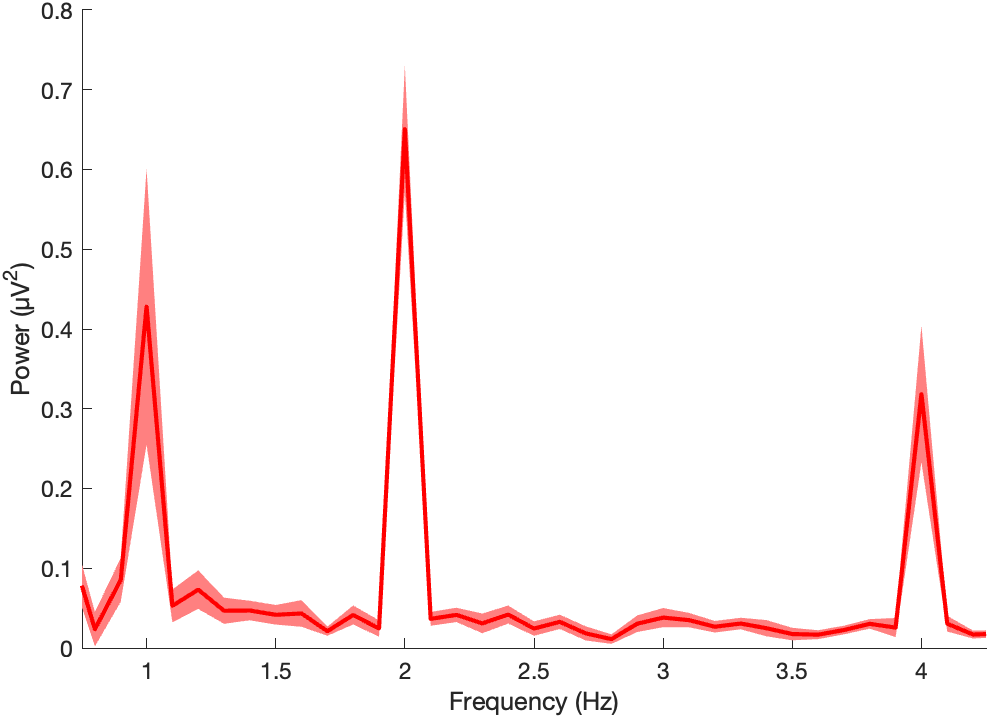
\includegraphics[width=0.95\linewidth]{figure/fig1.png}
    \captionsetup{labelsep=period}
    \caption{\small\rm 脑电信号的频谱图。脑电频谱(通道Cz)在句子、短语和音节频率(分别为1、2和4 Hz)处显示出三个幅度相似的峰值}
    \label{fig:fig1}

\end{figure}

\section{方法}

\begin{figure*}[!htb]
    \centering
    \begin{minipage}{0.49\textwidth}
        \centering
        \subcaption{}
        \vspace{-0.5em}
        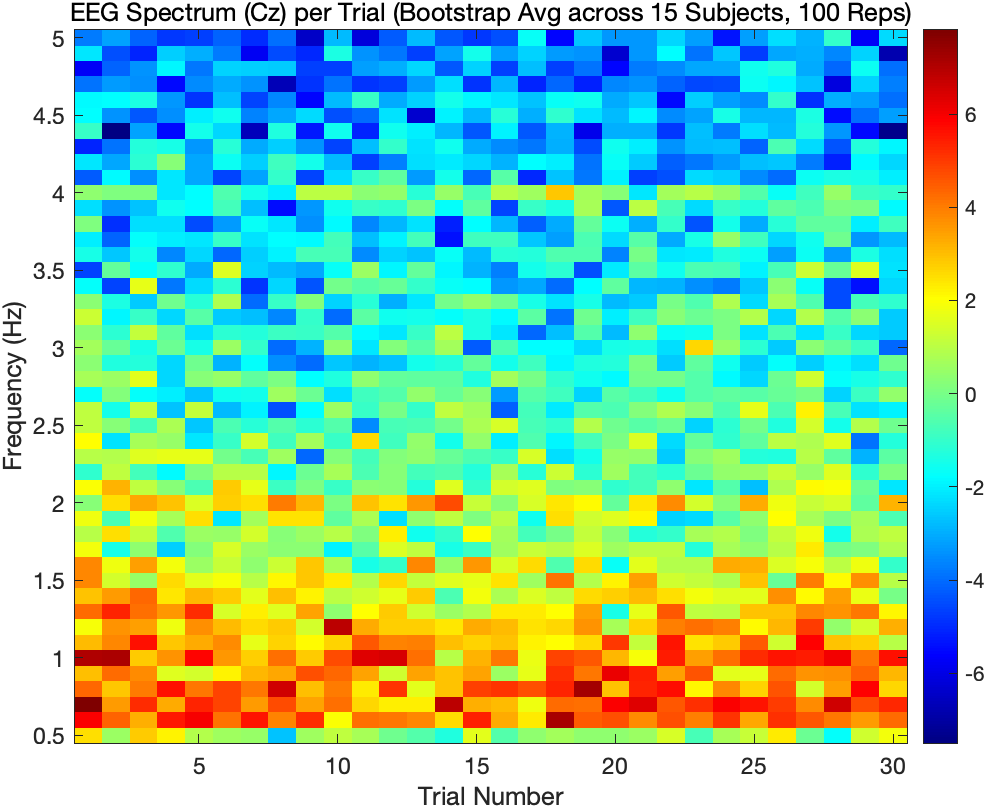
\includegraphics[width=\textwidth]{figure/fig2.png}
        \label{fig:fig2a}
    \end{minipage}
    \begin{minipage}{0.49\textwidth}
        \centering
        \subcaption{}
        \vspace{-0.5em}
        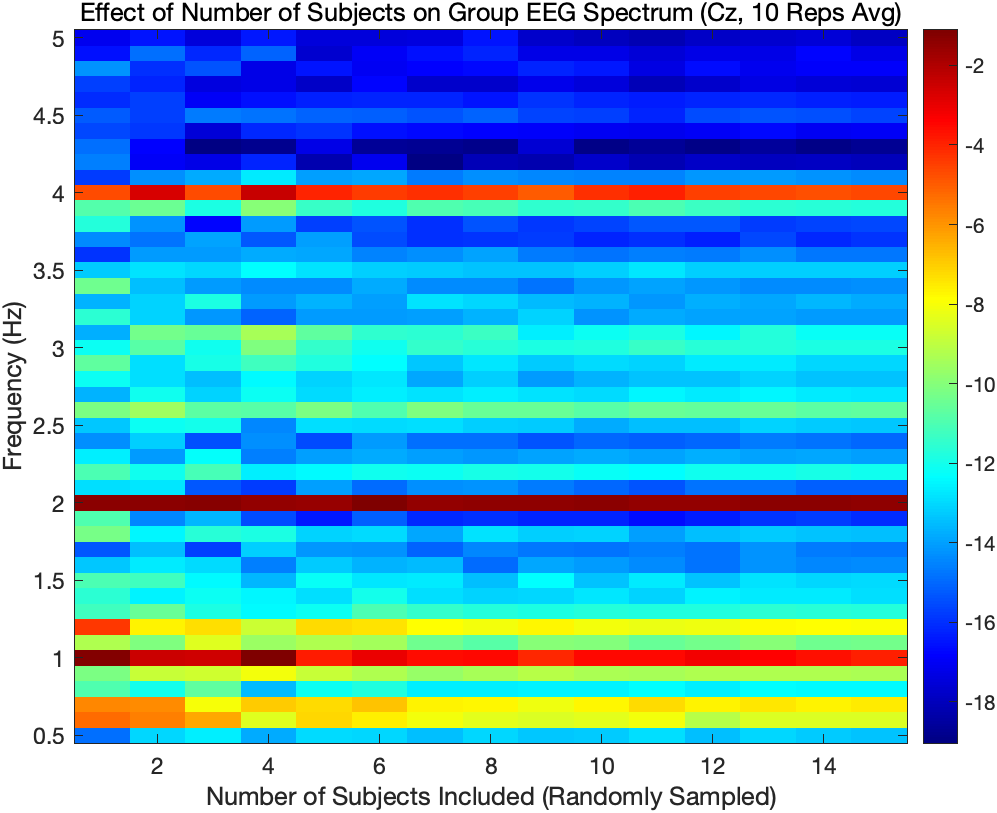
\includegraphics[width=\textwidth]{figure/fig3.png}
        \label{fig:fig2b}
    \end{minipage}
    \captionsetup{labelsep=period}
    \caption{\small\rm (a)逐试次各频率功率变化(Cz通道)。该图展示了单个试次间群体平均功率谱的变异性。横轴为试次序号(从1到30),纵轴为频率(Hz),范围为0.5Hz至5Hz。颜色强度:表示功率谱密度,单位为分贝(dB,相对于1μV²/Hz)。颜色越亮表示该频率点的功率越高。每个试次的数据是通过对该试次的15名被试数据进行Bootstrap(N=100)计算得到的群体几何平均频谱,再对这100次结果进行算术平均得到的最终估计值。(b)被试数量对群体EEG功率谱的影响(Cz通道)。该图展示了随着纳入分析的被试数量增加,群体平均功率谱的收敛情况。横轴为纳入分析的被试数量(从1到15)。图中每一列(对应被试数量m)的结果,是10次随机抽样平均得到的:每次抽样无放回地选取m名被试,计算这m名被试(基于其试次平均数据)的几何平均功率谱,最后将10次抽样的结果进行算术平均,作为包含m名被试时的群体频谱估计。}
\end{figure*}
\subsection{\heiti 数据采集}

本实验采用了\textcite{jin2018eye}实验1中的EEG数据。该实验记录了15名健康被试的EEG信号,每名被试完成了30个试次。每个试次包括播放了12个不同的句子,共48个音节,每个句子由4个音节组成,其中前两个音节构成名词短语,后两个音节构成动词短语。每个音节的持续时间为250ms。这些音节按照句子、短语和音节的层级结构组织,以便在不同层级上分析神经活动的追踪情况。EEG信号的采样率为2048 Hz,硬件低通滤波器设置为400 Hz以下。

EEG信号使用Biosemi ActiveTwo系统记录,配备64个依照国际10-20系统排布的Ag/AgCl电极。同时,记录了用于监测眼动的垂直和水平眼电图(EOG)信号。左右乳突处放置了额外电极,其平均信号在离线分析中用作参考电极。所有信号以2048 Hz的采样率进行采集,硬件低通滤波设置为400 Hz以下。

\subsection{\heiti 数据处理}

首先将EEG数据重参考至左右乳突电极的平均信号,然后采用线性相位有限脉冲响应(FIR)滤波器对EEG数据进行高通滤波,滤除0.7 Hz以下的低频成分。从每个EEG通道中去除水平和垂直EOG信号的影响,以校正眼动伪迹;将数据中偶然出现的大幅值的样本点置零。接着,为聚焦于低于4 Hz的目标低频响应并减少计算量,数据被降采样至16 Hz。

为了分析神经活动对不同语言层级结构的追踪情况,进行一下频谱分析。为避免刺激开始和结束时的瞬态响应,并侧重于稳态活动,选取每个12秒试次中间的10秒数据段(对应刺激呈现的第1秒至第11秒)用于分析。分析主要集中在中央顶叶的Cz电极。对每个被试在Cz通道上的10秒EEG数据段应用快速傅里叶变换(FFT),将其转换至频域。计算FFT结果的幅值平方,并进行适当缩放,得到单边功率谱密度(单位:μV²)。计算所有被试在Cz通道上的平均功率谱,并用Bootstrap方法重采样1000次,估计群体几何平均功率谱的标准误。

在探究试次和被试数量对脑电频率相应的影响时,分别对试次和被试数量进行了模拟。对于试次的影响,通过随机抽样和重复平均的方法,模拟了不同试次下的群体平均频谱。对于被试数量的影响,也通过随机抽样和重复平均的方法,模拟了不同被试数量下的群体平均频谱。具体可见图 \ref{fig:fig2a} 和图 \ref{fig:fig2b}的图注。

\section{结果}

\subsection{\heiti 脑电数据频谱分析结果复现}


如图 \ref{fig:fig1} 所示,群体平均的脑电功率谱清晰地展示了三个显著的峰值,分别位于1 Hz、2 Hz和4 Hz。这三个频率精确对应于实验刺激中嵌套的语言结构层级:1 Hz对应句子的呈现速率,2 Hz对应短语的呈现速率,而4 Hz则对应基础音节的呈现速率。三个峰值的幅度大致相当,这一特征也与\textcite{jin2018eye}报告的结果一致。





其中,4 Hz峰值的出现表明大脑对声音刺激中物理存在的音节节律产生了稳定的神经追踪响应。更为关键的是,1 Hz和2 Hz峰值的存在。由于实验中的语音流在物理上仅以恒定的4 Hz速率呈现音节,并不直接包含1 Hz或2 Hz的声学节律,这两个峰值的出现有力地证明了大脑神经活动能够超越刺激的物理属性,主动追踪并同步到由听者在认知层面构建出来的、更高层级的抽象语言结构(即句子和短语)。这一结果成功复现了原始研究的关键发现,证实了大脑在处理连续语音时对层级化语言结构的神经编码机制,

\subsection{\heiti 试次对频谱分析结果的影响}


各频率功率随试次变化的如图 \ref{fig:fig2a} 所示。从图中可以观察到试次间的变异性较大。虽然在目标频率1 Hz、2 Hz和4 Hz附近隐约可见能量相对较高的带状区域(图中偏红/黄色区域),但这些响应的强度和清晰度在不同试次间存在很大差异。例如,1 Hz的响应在某些试次(如第1、11、12个试次附近)表现得较为突出,而在其他试次则相对微弱或模糊。2 Hz和4 Hz的响应也呈现出类似的高度不稳定性。整体来看,图中并未显示出随着试验进行,某个频率的响应强度或模式发生系统性的增强或减弱的明显趋势。这表明,尽管平均来看大脑能够追踪这些语言结构,但在单个试验的层面上,神经响应的信噪比较低,且受到各种随机因素的影响,导致结果具有很大的波动性。因此,为了获得稳定可靠的频谱特征,对多个试次的数据进行平均是必要的。

\subsection{\heiti 被试数量对频谱分析结果的影响}

各频率功率随被试数增长的变化如图 \ref{fig:fig2b} 所示。图中清晰地揭示了纳入分析的被试数量对群体平均EEG功率谱结果的显著影响。当只包含少量被试时(图左侧),整个频谱波动较大,虽然目标频率(1 Hz, 2 Hz, 4 Hz)的峰值比较明显,但是其他频率的相应也较强。随着纳入分析的被试数量逐渐增加(从左到右),在1 Hz、2 Hz和4 Hz处的功率逐渐清晰和稳定,而其他频率的相应变得稳定且稳定。尤其是在包含接近或达到15名被试时(图右侧),这三个频率的峰值非常突出,与其他频率的背景噪声(蓝色区域)形成了鲜明对比。这表明,个体间的神经响应模式虽然存在差异,但通过对足够数量被试的数据进行平均(此处通过随机抽样和重复平均模拟),可以有效地提取出共同的、与任务相关的神经活动特征,同时抑制掉个体特异性的或随机的噪声成分。结果强调了足够的被试样本量对于获得可靠、可重复的群体水平神经影像学(尤其是EEG频谱)结果至关重要。


\printbibliography[title={\heiti 参\ 考\ 文\ 献}]

\end{document}

